\chapter{Implementation} \label{cha:implementation}
	The Bachelor Project course would not be a real Bachelor Project course if 
	there were projects without technical challenges whatsoever regarding the 
	implementation of the final result. Therefore, this chapter elaborates
	on the technical challenges faced during development of the project and
	the solutions that we have developed for these challenges.
	%TODO Highlight technical challenges and elaborate on solutions for these challenges.
	%     This includes (amongst others) how the AR functionality posed a problem and we
	%     implemented a C++ server using OpenCV to take over that work (along with 
	%     synchronizing on a central camera).
	
	% Sections are purely by example. This list might not be entirely correct or complete.
	\section{AR Glasses} \label{sec:arglasses}
		One of the first design choices that we had to make was about what
		AR glass was going to be used with the project. As can be seen in
		our research report, under appendix \ref{app:researchreport},
		there two options to choose from. These were the Oculus and
		the META One. We eventually settled for the META One, because
		of the latency of the Oculus. A pair of META Glasses can be seen in
		figure \ref{fig:metaone}.
		
		\begin{figure}[!ht]
			\centering
			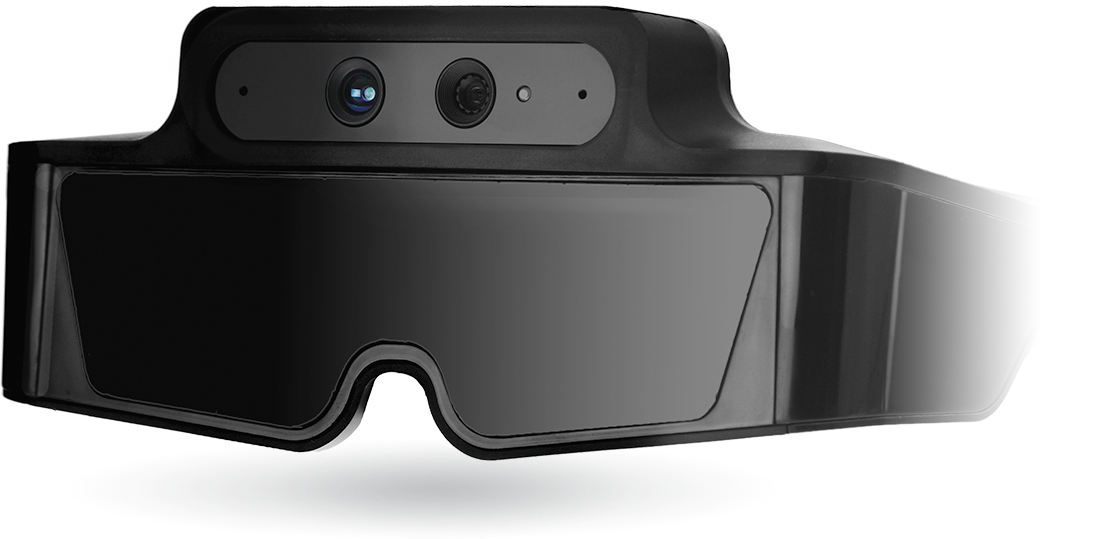
\includegraphics[width=\textwidth]{MetaOneGlasses}
			\caption{A pair of META One glasses.}
			\label{fig:metaone}
		\end{figure}
		
		The challenge with the META One was to get it working in Unity.
		There is a Meta SDK which allows for Unity games to work with
		the META One, but AR itself is still in development (as of
		writing this report), and the META One glasses are experimental
		at best. The SDK that we used first was also very buggy (due to the
		experimental nature of the META One).
		
		\subsection{SLAM tracking} \label{ssec:slamloc}
			SLAM is an acronym, which stands for Simultaneous Localization And
			Mapping. It stands for a computational problem involving making
			a map of an unknown environment while updating the location of
			the agent within it (this definition follows from Wikipedia).
			

	\section{Marker Detection} \label{sec:markerdetection}
		...
		
	\section{Synchronization of World State} \label{sec:synchronization}
		...
		
	\section{Networking and the OpenCV server} \label{sec:network}
		...
	